\documentclass[palatino,nochap]{apuntes}

\title{Comentarios sobre los otros ejercicios}
\author{Daniel Ruiz Mayo, Alberto Javier Parramón, Víctor de Juan}
\date{}

% Paquetes adicionales

% --------------------

\begin{document}
\pagestyle{plain}
\maketitle

% Contenido.

%% Apéndices (ejercicios, exámenes)
%\appendix

\section{Ejercicio 2}

El algoritmo de PageRank lo hemos implementado de forma matricial, utilizando la librería \href{http://ejml.org/wiki/index.php?title=Main_Page}{ejml} (\textit{Efficient Java Matrix Library})

La implementación matricial del algoritmo la estudiamos en la asignatura \textit{Modelización} del grado en Matemáticas y hemos utilizado los apuntes (\href{https://www.dropbox.com/sh/kbymf37cykz77ha/AACL44kNShOUqhALNNnjdmcoa/modelizacion.pdf?dl=0}{[Valero,2015]}) de la asignatura para la implementacíon del algoritmo.
 \newpage
\section{Ejercicio 3}



Para este crawler hemos usado como web de referencia wikipedia, y hemos tomado 100 paginas, generando un fichero llamado graph.txt con las urls salientes de estas 100 páginas.
Si se quiere ejecutar, requiere un proceso manual, debido a que no se ha conseguido automatizar la creación de un zip en el que se incluyeran todos los html de la carpeta WEBCRAWLER sin que apareciera esta carpeta dentro del docs.zip.
Se requiere una primera ejecución para descargar todos los documentos html y una vez realizada comprimir todos los archivos de la carpeta WEBCRAWLER en una zip llamado docs.zip

Como podemos ver en pagerank.txt las páginas con mayor score son 

\begin{table}
	\begin{tabular}{cc}
		\verb|https://es.wikipedia.org/wiki/Miner%C3%ADa\_de\_datos| & 5.659309564233164E-4 \\ \verb|https://es.wikipedia.org/wiki/Tratamiento\_de\_base\_de\_datos| & 5.659309564233164E-4 \\
		\verb|https://es.wikipedia.org/wiki/Inteligencia\_artificial| & 5.659309564233164E-4 \\
		\verb|https://es.wikipedia.org/wiki/Variable\_dependiente| & 5.659309564233164E-4 \\
		\verb|https://es.wikipedia.org/wiki/Histograma| & 5.659309564233164E-4 \\
		\verb|https://es.wikipedia.org/wiki/Mapa\_autoorganizado| & 5.659309564233164E-4 \\
		\verb|https://es.wikipedia.org/wiki/M%C3%A1quina\_oracle| & 5.659309564233164E-4 \\
		\verb|https://es.wikipedia.org/wiki/Ciencia| & 5.659309564233164E-4 \\
		\verb|https://es.wikipedia.org/wiki/Gen%C3%A9tica| & 5.659309564233164E-4 \\
		\verb|https://es.wikipedia.org/wiki/Ingenier%C3%ADa\_el%C3%A9ctrica| & 5.659309564233164E-4 \\
	\end{tabular}
	\caption{Top 10 de páginas con mayor puntuación}
\end{table}

Por otra parte los resultados a la consulta Minería de datos en el indice son los que se ven en la imagen.

\begin{figure}
	\centering
	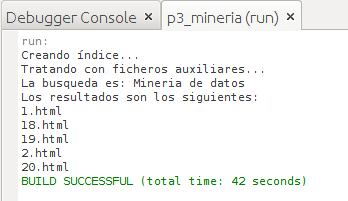
\includegraphics[scale=0.7]{Salida_crawler.png}
	\caption{Resultados para la consulta "Minería de datos"}
\end{figure}

Estas páginas no nos sorprenden, pues corresponden a las páginas de wikipedia de Minería de datos, Tratamiento de base de datos,R (lenguaje de programación), SPSS y RapidMiner.
Como detalle decir que si buscamos minería de datos en Google la primera opción es la misma que la nuestra, la pagina de mineria de datos de wikipedia.

\end{document}
